\newcommand{\RequiredPeers}{\ensuremath{N_\mathit{rs}}}

% TODO: once verified, mark all these things are "not in the paper, but verified
% by the researchers"
\newcommand{\VerifiedByResearchers}{\todo{Verify}}

\chapter{Ouroboros Genesis}
\label{genesis}

\section{Introduction}

\subsection{Background: understanding the Longest Chain rule}
\label{genesis:background:longest-chain}

Recall the Praos chain selection rule:

\begin{definition}[Longest Chain Rule]
\label{longest-chain-rule}
A candidate chain is preferred over our current chain if
%
\begin{enumerate}
\item it is longer than our chain, and
\item the intersection point is no more than $k$ blocks away from our tip.
\end{enumerate}
\end{definition}

The purpose of chain selection is to resolve temporary forks that arise from the
normal operation of the protocol (such as when there are multiple leaders in a
single slot), and---importantly---to distinguish honest chains from chains
forged by malicious nodes. It is not a priori clear why choosing longer chains
over shorter chains would help distinguish malicious chains from honest chains:
why would an honest chain be longer?

Recall that the leadership schedule is based on stake: a node's probability of
being elected a leader in a given slot is proportional to their stake. By
assumption, the malicious nodes in the system together have less stake than the
honest nodes; security of the system as a whole critically depends on the
presence of this honest majority. This means that when a malicious node extends
the chain they can only produce a chain with relatively few filled slots: the
honest chain will be \emph{denser}. At least, this will be true near the
intersection point: as we get further away from that intersection point, the
malicious node can attempt to influence the leadership schedule for future slots
to their advantage.

The Praos security analysis \cite{cryptoeprint:2017:573} tells us that provided
all (honest) nodes are online all the time, they will all share the same chain,
except for blocks near the tips of those chains. Moreover, blocks with a slot
number ahead of the wall clock are considered invalid. This means that the only
way\footnote{The chain sync client does actually allow for some clock skew.
Headers that exceed the clock skew should not be taking into account in the
calculations that we discuss in this chapter.} for one chain to be longer than
another is by having more filled slots between the tip of the shared prefix and
``now'': in other words, they must be \emph{denser}.
%
\begin{center}
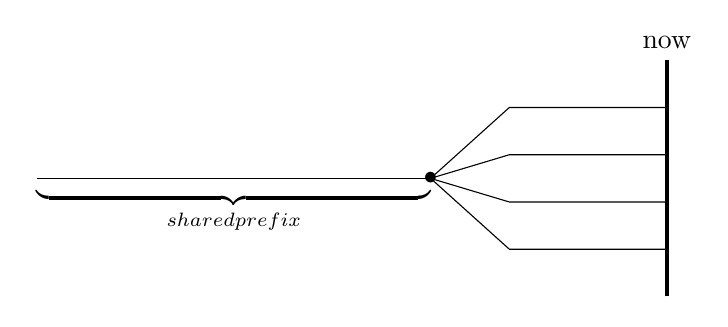
\begin{tikzpicture}
\draw (0,0) -- (5,0) coordinate(branch) node{$\bullet$} node[pos=0.5,below]{$\underbrace{\hspace{5cm}}_\text{shared prefix}$};
\draw (branch) -- ++(1,  0.9) -- ++(2,0);
\draw (branch) -- ++(1,  0.3) -- ++(2,0);
\draw (branch) -- ++(1, -0.3) -- ++(2,0);
\draw (branch) -- ++(1, -0.9) -- ++(2,0);
\draw [ultra thick] (8,-1.5) -- (8,1.5) node[above]{now};
\end{tikzpicture}
\end{center}
%
This motivates the first part of the Longest Chain rule: chain length is a
useful proxy for chain density. The second part of the rule---the intersection
point is no more than $k$ blocks away from our tip---is important because we can
only meaningfully compare density \emph{near the intersection point}. As
we get further away from the intersection point, the attacker can start to
influence the leadership schedule. This means that if the attacker's chain
forks off from the honest chain far back enough, they can construct a chain
that is longer than the honest chain. The side condition to the Longest Chain
rule means that we will simply not even consider chains that fork off that
far back.We can still resolve minor forks that happen in the honest chain during
the normal operation of the protocol, because---so the metatheory
guarantees---those will not be deeper than $k$ blocks.

\subsection{Nodes joining late}

When new nodes join the network (or rejoin after having been offline for a
while), they don't have the advantage of having been online since the start of
the system, and have no sufficiently long prefix of the honest chain available.
As we saw at the end of \cref{genesis:background:longest-chain}, simply looking
at chain length is insufficient to distinguish the honest chain from malicious
chains: given enough time, an attacker can produce a chain that is longer than
the honest chain:
%
\begin{center}
\begin{tikzpicture}
\draw (-2,0) node{$\bullet$} -- (0,0);
\draw (0,0) node{$\bullet$} -- (6,0) node{$\bullet$} node[right] {honest chain};
\draw (0,0) -- (0,-1) -- (8,-1) node{$\bullet$} node[right]{attacker's chain};
\path (0,0) -- (6,0) node[pos=0.5, above=0.5]{$\overbrace{\hspace{6cm}}^{\text{$\gg k$ blocks}}$};
\end{tikzpicture}
\end{center}
%
When a node's current chain is somewhere along that commom prefix and uses the
longest chain rule, they will choose the attacker's chain rather than the honest
chain. Moreover, they will now never switch to the honest chain, because the
intersection point with that chain is more than $k$ blocks ago. If a node would
get a ``leg up'' in the form of a reliable message telling which chain to adopt
when joining the network (such a message is known as a ``checkpoint'' in the
consensus literature), the Praos rule from that point forward would prevent them
from (permanently) adopting the wrong chain, but Praos cannot be used to help
nodes ``bootstrap'' when they are behind.

So far we have just been discussing Praos as it is described in theory. The
situation in practice is worse. In the abstract models of the consensus
algorithm, it is assumed entire chains are being broadcast and validated. In
reality, chains are downloaded and validated one block at a time.
We therefore don't see a candidate chain's \emph{true} length; the length of a
candidate we see depends on how much of that candidate's chain we have
downloaded\footnote{Nodes do report their ``true length'', but since we have no
way of verifying this information until we have seen the entire chain, we can
make no use of this information for the purpose of chain selection.}. Defining
chain selection in terms of chain length, where our \emph{perceived} chain
length depends on what we decide to download, is obviously rather circular.
In terms of the above discussion, it means that the attacker's chain doesn't
even need to be longer than the honest chain:
%
\begin{center}
\begin{tikzpicture}
\draw (-2,0) node{$\bullet$} -- (0,0);
\draw (0,0) node{$\bullet$} -- (10,0) node{$\bullet$} node[right] {honest chain};
\draw (0,0) -- (0,-1) -- (4,-1) node{$\bullet$} node[right]{attacker's chain};
\path (0,0) -- (4,0) node[pos=0.5, above=0.5]{$\overbrace{\hspace{4cm}}^{\text{$> k$ blocks}}$};
\end{tikzpicture}
\end{center}
%
If the attacker's chain contains more than $k$ blocks after the intersection
point, and we \emph{happen} to download that chain first, we would adopt it and
subsequently be unable to switch to the honest chain, since that would involve a
rollback of more than $k$ blocks, which the Praos rule forbids.

\subsection{The Density rule}

It is therefore clear we need a different chain selection rule, and the
Ouroboros Genesis paper \cite{cryptoeprint:2018:378} proposes one:
%
\begin{definition}[Density Rule]
A candidate chain is preferred over our current chain if it is denser
(contains more blocks) in a window of $s$ slots anchored at the intersection
between the two chains.
\end{definition}
%
(We will refer to this as the Density rule, rather than the Genesis rule,
because the rule as we will present in in this chapter is dfferent from, though
equivalent to, the rule as it presented in the paper.\VerifiedByResearchers{}).
Technically speaking, $s$ is a parameter of the rule, but in practice we will
want to set it to be equal to the stability window:\VerifiedByResearchers{}

\begin{definition}[Genesis window size]
The genesis window size $s$ must be set to $s = 3k/f$.
\end{definition}

As it turns out, for nodes that are up to date, this new rule does not change
how chain selection works:

\begin{lemma}[Rule Equivalence]
\label{rule-equivalence}
When comparing two chains that only differ in the last $k$ blocks, the
Density rule and the Longest Chain rule are equivalent.
\end{lemma}

\begin{proof}[Proof (sketch)]
The two chains differ only in the last $k$ blocks; since $s$ slots will contain
at least $k$ blocks, the fragments of the chain after the intersection point
will not exceed $s$ slots:
%
\begin{center}
\begin{tikzpicture}
\draw (0,0) -- (6,0) coordinate (I);
\path (I) -- ++(0,1) -- ++(3,0) node[pos=0.5,above=0.1]{$\overbrace{\hspace{3cm}}^\text{$\le k$ blocks}$};
\draw (I) -- ++(1,1) -- ++(1.5,0);
\draw (I) -- ++(1,-1) -- ++ (2,0);
\draw [dashed]
    (I)
  -- ++(0, 2)
  -- ++(4, 0) node[pos=0.5,above]{$s$ slots}
  -- ++(0, -3.5)
  -- ++(-4, 0)
  -- cycle;
\end{tikzpicture}
\end{center}
%
This means that density within the window indeed is just chain length.
\end{proof}

Unlike the Longest Chain rule, the Density rule does not impose a maximum
rollback. It does not need to, as it always considers density \emph{at the
intersection point}. From an implementation perspective, this is useful;
in a situation such as
%
\begin{center}
\begin{tikzpicture}
\draw (-2,0) node{$\bullet$} -- (0,0);
\draw (0,0) node{$\bullet$} -- (10,0) node{$\bullet$} node[right] {honest chain};
\draw (0,0) -- (0,-1) -- (4,-1) node{$\bullet$} node[right]{attacker's chain};
\path (0,0) -- (4,0) node[pos=0.5, above=0.5]{$\overbrace{\hspace{4cm}}^{\text{$> k$ blocks}}$};
\end{tikzpicture}
\end{center}
%
if we happen to see and adopt the attacker's chain first, and then later find
the honest chain, we can still adopt the honest chain (which will be denser at
the intersection point, because of the honest majority). However, this  would
involve a rollback of more than $k$ blocks. This is problematic for consensus;
we depend on this maximum rollback in many ways
(\cref{consensus:overview:k,storage:components,chainsyncclient:validation,chainsyncclient:forecasting}
and others), and we will want to \emph{continue} to depend on it. Less
fundamentally, but nonetheless importantly, it also doesn't fit very well with
our look-at-the-tip-only approach (\cref{consensus:overview:chainsel}). The
resolution of this problem is the subject of this chapter.

\section{Local versus global chain selection}







\pagebreak


\debugsep{OLD}

\section{Introduction}

\subsection{Chain length versus chain density}
\label{genesis:intro:length-vs-density}

%
Conversely, the density of the fragment of a chain is only meaningful if that
fragment is long enough. Since the leadership election is a probabilistic
process, we only expect fragments to contain more slots signed by honest nodes
\emph{on average}, and we can only draw conclusions from density on long enough
fragments.

\subsection{Speculative mode}

Chain selection so far has been running in what we might call a ``speculative''
mode: when we see a new chain, we compare it to our current chain, and if we
prefer it, we adopt it (\cref{speculative-chain-selection}). This is speculative
in the sense that if we later see a second chain, we can change our mind about
adopting the first and adopt the second if that second chain is preferred over
the first.


\begin{figure}[p]
\hrule

\begin{tabular}{ll@{$\quad\Rightarrow\quad$}l}

(a)
&
&
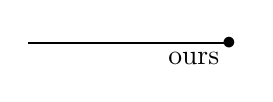
\begin{tikzpicture}[xscale=0.85]
\path (0, 0) coordinate (tip) node{$\bullet$} node[below left]{ours};
\draw (tip) + (-3,0) -- (tip);
\end{tikzpicture}
\\[1em]

(b)
&
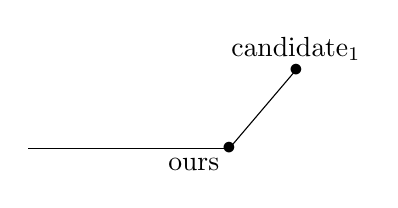
\begin{tikzpicture}[xscale=0.85]
\path (0, 0) coordinate (tip) node{$\bullet$} node[below left]{ours};
\draw (tip) + (-3,0) -- (tip);
\draw (tip) -- ++(1.0,  1.0) node{$\bullet$} coordinate (ab) node[above]{candidate$_1$};
\end{tikzpicture}
&
\begin{tikzpicture}[xscale=0.85]
\path (0, 0) coordinate (tip) node{$\bullet$};
\draw (tip) + (-3,0) -- (tip);
\draw (tip) -- ++(1.0,  1.0) node{$\bullet$} coordinate (ab) node[above]{ours};
\end{tikzpicture}
\\[1em]

(c)
&
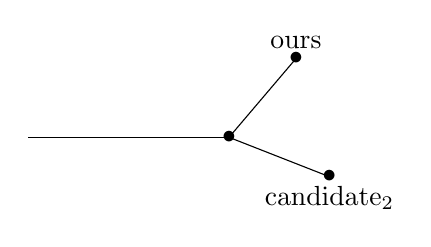
\begin{tikzpicture}[xscale=0.85]
\path (0, 0) coordinate (tip) node{$\bullet$};
\draw (tip) + (-3,0) -- (tip);
\draw (tip) -- ++(1.0,  1.0) node{$\bullet$} coordinate (ab) node[above]{ours};
\draw (tip) -- ++(1.5, -0.5) coordinate (cd) node{$\bullet$} node[below]{candidate$_2$};
\end{tikzpicture}
&
\begin{tikzpicture}[xscale=0.85]
\path (0, 0) coordinate (tip) node{$\bullet$};
\draw (tip) + (-3,0) -- (tip);
\draw (tip) -- ++(1.0,  1.0) node{$\bullet$} coordinate (ab);
\draw (tip) -- ++(1.5, -0.5) coordinate (cd) node{$\bullet$} node[below]{ours};
\end{tikzpicture}
\\[1em]

(d)
&
\begin{tikzpicture}[xscale=0.85]
\path (0, 0) coordinate (tip) node{$\bullet$};
\draw (tip) + (-3,0) -- (tip);
\draw (tip) -- ++(1.0,  1.0) node{$\bullet$} coordinate (ab);
\draw (tip) -- ++(1.5, -0.5) coordinate (cd) node{$\bullet$} node[below]{ours};
\draw (ab) -- ++(0.5,  0.5) -- ++(2.0, 0) node{$\bullet$} node[above]{candidate$_3$};
\end{tikzpicture}
&
\begin{tikzpicture}[xscale=0.85]
\path (0, 0) coordinate (tip) node{$\bullet$};
\draw (tip) + (-3,0) -- (tip);
\draw (tip) -- ++(1.0,  1.0) node{$\bullet$} coordinate (ab);
\draw (tip) -- ++(1.5, -0.5) coordinate (cd) node{$\bullet$};
\draw (ab) -- ++(0.5,  0.5) -- ++(2.0, 0) node{$\bullet$} node[above]{ours};
\end{tikzpicture}
\\[1em]

(e)
&
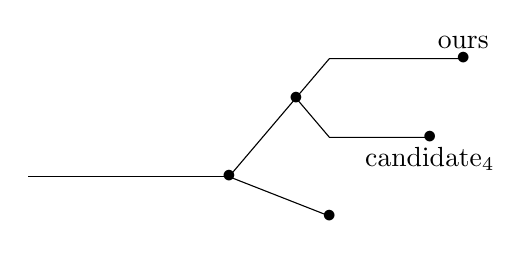
\begin{tikzpicture}[xscale=0.85]
\path (0, 0) coordinate (tip) node{$\bullet$};
\draw (tip) + (-3,0) -- (tip);
\draw (tip) -- ++(1.0,  1.0) node{$\bullet$} coordinate (ab);
\draw (tip) -- ++(1.5, -0.5) coordinate (cd) node{$\bullet$};
\draw (ab) -- ++(0.5,  0.5) -- ++(2.0, 0) node{$\bullet$} node[above]{ours};
\draw (ab) -- ++(0.5, -0.5) -- ++(1.5, 0) node{$\bullet$} node[below]{candidate$_4$};
\end{tikzpicture}
&
\begin{tikzpicture}[xscale=0.85]
\path (0, 0) coordinate (tip) node{$\bullet$};
\draw (tip) + (-3,0) -- (tip);
\draw (tip) -- ++(1.0,  1.0) node{$\bullet$} coordinate (ab);
\draw (tip) -- ++(1.5, -0.5) coordinate (cd) node{$\bullet$};
\draw (ab) -- ++(0.5,  0.5) -- ++(2.0, 0) node{$\bullet$} node[above]{ours};
\draw (ab) -- ++(0.5, -0.5) -- ++(1.5, 0) node{$\bullet$};
\end{tikzpicture}
\\[1em]

(f)
&
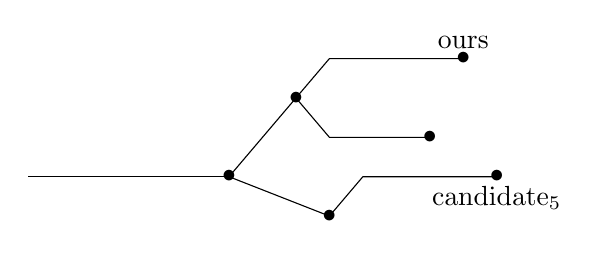
\begin{tikzpicture}[xscale=0.85]
\path (0, 0) coordinate (tip) node{$\bullet$};
\draw (tip) + (-3,0) -- (tip);
\draw (tip) -- ++(1.0,  1.0) node{$\bullet$} coordinate (ab);
\draw (tip) -- ++(1.5, -0.5) coordinate (cd) node{$\bullet$};
\draw (ab) -- ++(0.5,  0.5) -- ++(2.0, 0) node{$\bullet$} node[above]{ours};
\draw (ab) -- ++(0.5, -0.5) -- ++(1.5, 0) node{$\bullet$};
\draw (cd) -- ++(0.5,  0.5) -- ++(2.0, 0) node{$\bullet$} node[below]{candidate$_5$};
\end{tikzpicture}
&
\begin{tikzpicture}[xscale=0.85]
\path (0, 0) coordinate (tip) node{$\bullet$};
\draw (tip) + (-3,0) -- (tip);
\draw (tip) -- ++(1.0,  1.0) node{$\bullet$} coordinate (ab);
\draw (tip) -- ++(1.5, -0.5) coordinate (cd) node{$\bullet$};
\draw (ab) -- ++(0.5,  0.5) -- ++(2.0, 0) node{$\bullet$};
\draw (ab) -- ++(0.5, -0.5) -- ++(1.5, 0) node{$\bullet$};
\draw (cd) -- ++(0.5,  0.5) -- ++(2.0, 0) node{$\bullet$} node[below]{ours};
\end{tikzpicture}
\\
\end{tabular}

\hrule
\caption{\label{speculative-chain-selection}Speculative chain selection}
\end{figure}

\subsection{Genesis rule}



\begin{definition}[Genesis window size]
\label{default-genesis-window}
The genesis window size $s$ must be equal to the stability window;
that is $s = 3k / f$.
\end{definition}

The genesis rule we will use in this chapter differs slightly from the one from
the original paper:

\begin{definition}[Genesis rule]
\label{genesis:rule}
A candidate chain is preferred over our current chain if

\begin{itemize}
\item The intersection between the candidate chain and our chain is \textbf{at
least $s$ slots} back from the tip of our chain, and the candidate chain is
\textbf{denser} in a window of $s$ slots at the intersection, or

\item The intersection between the candidate chain and our chain is \textbf{less
than $s$ slots} back from the tip of our chain, and the candidate chain is
strictly \textbf{longer} than our chain.
\end{itemize}

\end{definition}

\subsection{Conservative mode}
\label{genesis:intro:conservative}


Specifically, we will switch from the default speculative chain selection mode
to a \emph{conservative} chain selection mode. We will see the details of how
this mode works later in this chapter, but the intuition is that rather than
considering and possibly adopting chains as we encounter them, we instead wait,
collecting enough information to fill a ``look-ahead window'' which will allow
us to make progress, either discarding candidates or adopting blocks.
Critically, the decisions we make in conservative mode are not subject to
rollback: we wait until we can be sure. \Cref{conservative-chain-selection}
illustrates what this might look like.

The security analysis of the genesis chain selection rule includes a theorem
\cite[Theorem 2]{cryptoeprint:2018:378} that says that it is still true that
\emph{when nodes are up to date} they will never need to roll back more than $k$
blocks. We can use this theorem to justify switching from the conservative
mode back to the speculative mode. Since blocks ahead of the wall clock are
considered invalid, we can use the current slot number (according to the
wallclock) to estimate if we are within $k$ blocks from the longest chain
in the network. We cannot do better than an estimate because we might not know
the density of that chain. The latest point we can switch is $s$ slots away
from the wall clock: any later and we would not be able to look-ahead far enough
to apply the genesis rule (see \cref{genesis:rules}, especially
\cref{{genesis:insufficient-blocks}}). As it turns out, we will need to switch a
little sooner than that; we will discuss the details in
\cref{genesis:insufficient-blocks,genesis:switch-over-point}.

The switch over point does not change the chain selection rule itself: even when
we are in speculative mode, we will still apply the genesis rule as defined in
\cref{genesis:rule}, comparing density or length depending on the intersection
point; we will merely use Theorem 2 of the genesis security analysis to justify
imposing the standard maximum rollback of $k$ blocks.

\begin{figure}[p]
\hrule

\begin{tabular}{ll@{$\quad\Rightarrow\quad$}l}
a &&
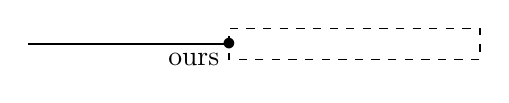
\begin{tikzpicture}[xscale=0.85]
\path (0, 0) coordinate (tip) node{$\bullet$} node[below left]{ours};
\draw [dashed] (tip) -- ++(0, 0.2) -- ++(3.75, 0) -- ++(0, -0.4) -- ++(-3.75, 0) -- cycle;
\draw (tip) + (-3,0) -- (tip);
\end{tikzpicture}
\\

b &&
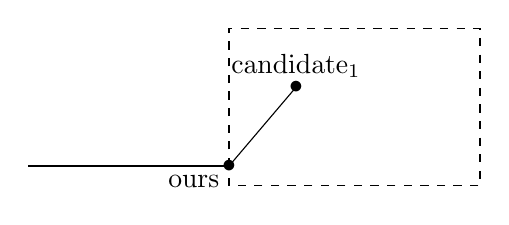
\begin{tikzpicture}[xscale=0.85]
\path (0, 0) coordinate (tip) node{$\bullet$} node[below left]{ours};
\draw [dashed] (tip) -- ++(0, 1.75) -- ++(3.75, 0) -- ++(0, -2) -- ++(-3.75, 0) -- cycle;
\draw (tip) + (-3,0) -- (tip);
\draw (tip) -- ++(1.0,  1.0) node{$\bullet$} coordinate (ab) node[above]{candidate$_1$};
\end{tikzpicture}
\\

c &&
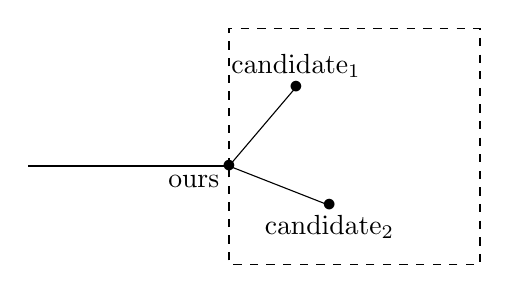
\begin{tikzpicture}[xscale=0.85]
\path (0, 0) coordinate (tip) node{$\bullet$} node[below left]{ours};
\draw [dashed] (tip) -- ++(0, 1.75) -- ++(3.75, 0) -- ++(0, -3) -- ++(-3.75, 0) -- cycle;
\draw (tip) + (-3,0) -- (tip);
\draw (tip) -- ++(1.0,  1.0) node{$\bullet$} coordinate (ab) node[above]{candidate$_1$};
\draw (tip) -- ++(1.5, -0.5) coordinate (cd) node{$\bullet$} node[below]{candidate$_2$};
\end{tikzpicture}
\\

d &&
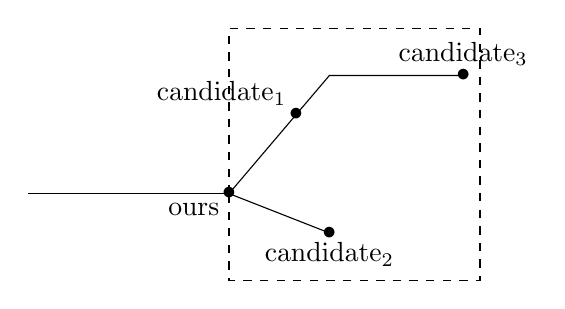
\begin{tikzpicture}[xscale=0.85]
\path (0, 0) coordinate (tip) node{$\bullet$} node[below left]{ours};
\draw [dashed] (tip) -- ++(0, 2.1) -- ++(3.75, 0) -- ++(0, -3.2) -- ++(-3.75, 0) -- cycle;
\draw (tip) + (-3,0) -- (tip);
\draw (tip) -- ++(1.0,  1.0) node{$\bullet$} coordinate (ab) node[above left]{candidate$_1$};
\draw (tip) -- ++(1.5, -0.5) coordinate (cd) node{$\bullet$} node[below]{candidate$_2$};
\draw (ab) -- ++(0.5,  0.5) -- ++(2.0, 0) node{$\bullet$} node[above]{candidate$_3$};
\end{tikzpicture}
\\

e &&
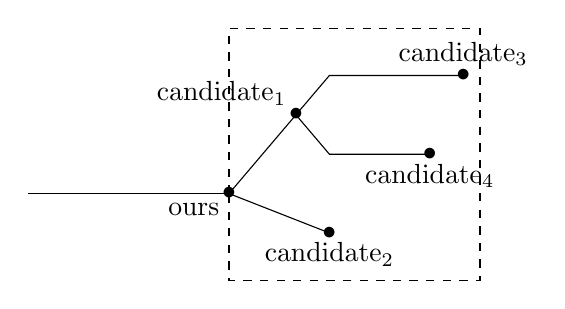
\begin{tikzpicture}[xscale=0.85]
\path (0, 0) coordinate (tip) node{$\bullet$} node[below left]{ours};
\draw [dashed] (tip) -- ++(0, 2.1) -- ++(3.75, 0) -- ++(0, -3.2) -- ++(-3.75, 0) -- cycle;
\draw (tip) + (-3,0) -- (tip);
\draw (tip) -- ++(1.0,  1.0) node{$\bullet$} coordinate (ab) node[above left]{candidate$_1$};
\draw (tip) -- ++(1.5, -0.5) coordinate (cd) node{$\bullet$} node[below]{candidate$_2$};
\draw (ab) -- ++(0.5,  0.5) -- ++(2.0, 0) node{$\bullet$} node[above]{candidate$_3$};
\draw (ab) -- ++(0.5, -0.5) -- ++(1.5, 0) node{$\bullet$} node[below]{candidate$_4$};
\end{tikzpicture}
\\

f &&
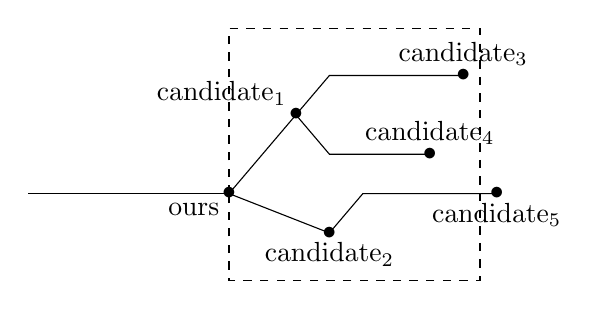
\begin{tikzpicture}[xscale=0.85]
\path (0, 0) coordinate (tip) node{$\bullet$}  node[below left]{ours};
\draw [dashed] (tip) -- ++(0, 2.1) -- ++(3.75, 0) -- ++(0, -3.2) -- ++(-3.75, 0) -- cycle;
\draw (tip) + (-3,0) -- (tip);
\draw (tip) -- ++(1.0,  1.0) node{$\bullet$} coordinate (ab) node[above left]{candidate$_1$};
\draw (tip) -- ++(1.5, -0.5) coordinate (cd) node{$\bullet$} node[below]{candidate$_2$};
\draw (ab) -- ++(0.5,  0.5) -- ++(2.0, 0) node{$\bullet$} node[above]{candidate$_3$};
\draw (ab) -- ++(0.5, -0.5) -- ++(1.5, 0) node{$\bullet$}  node[above]{candidate$_4$};
\draw (cd) -- ++(0.5,  0.5) -- ++(2.0, 0) node{$\bullet$} node[below]{candidate$_5$};
\end{tikzpicture}
\\

g &&
\begin{tikzpicture}[xscale=0.85]
\path (0, 0) coordinate (tip) node{$\bullet$};
\draw [dashed] (tip) -- ++(0, 2.1) -- ++(3.75, 0) -- ++(0, -3.2) -- ++(-3.75, 0) -- cycle;
\draw (tip) + (-3,0) -- (tip);
\draw [dotted] (tip) -- ++(1.0,  1.0) coordinate (ab);
\draw (tip) -- ++(1.5, -0.5) coordinate (cd) node{$\bullet$} node[below]{ours};
\draw [dotted] (ab) -- ++(0.5,  0.5) -- ++(2.0, 0);
\draw [dotted] (ab) -- ++(0.5, -0.5) -- ++(1.5, 0);
\draw (cd) -- ++(0.5,  0.5) -- ++(2.0, 0) node{$\bullet$} node[below]{candidate$_5$};
\end{tikzpicture}
\\

\end{tabular}

\hrule
\caption{\label{conservative-chain-selection}Conservative chain selection}
\end{figure}

\section{Applying the genesis rule in conservative mode}
\label{genesis:rules}

In this section we will show the rules that we will use to implement the
genesis chain selection rule whilst in conservative mode. Throughout we will
rely critically on the following assumption:

\begin{assumption}[Representative sample]
There exists some threshold $\RequiredPeers$ such that if we see the chains of
at least $\RequiredPeers$ peers, we have seen a representative sample of
\emph{all} relevant chains available in the network at that time; there are no
other chains in the network that we do not know about but \emph{should} know
about.
\end{assumption}

This implies that an attacker cannot \emph{eclipse} us; this is something
outside the scope of the consensus layer, and must be guaranteed by the network
layer (probably by a probabilistic way of choosing peers).

We will set the size of our ``look-ahead window'' to be precisely $s$; that is,
we will set the size of the look-ahead window used for conservative chain
selection to be exactly equal to the genesis window (we will see shortly why
this is a suitable choice). There are now two possibilities: either all chains
in our window share a common prefix, or they don't and they fork at the start of
the window. We will consider these two cases separately.

\pagebreak

\subsection{Fork: discard}
\label{genesis:discard}

Suppose that $\RequiredPeers = 4$, and our window looks like this:
%
\begin{center}
\begin{tikzpicture}[yscale=0.75]
\path (0, 0) coordinate (tip) node{$\bullet$} node[below left]{tip};
\draw (tip) -- ++(1.0,  1.0) coordinate (ab) node{$\bullet$} node[above left]{$ab$};
\draw [dotted] (tip) -- ++(1.5, -0.5) coordinate (cd);
\draw (ab) -- ++(0.5,  0.5) -- ++(2.0, 0) coordinate(A) node[right]{$A$};
\draw (ab) -- ++(0.5, -0.5) -- ++(2.0, 0) node[right]{$B$};
\draw [dotted] (cd) -- ++(0.5,  0.5) -- ++(1.5, 0) node[right]{$C$};
\draw [dotted] (cd) -- ++(0.5, -0.5) -- ++(1.5, 0) node[right]{$D$};
\draw [dashed]
     (tip)
  -- ++(0, 1.75)
  -- ++(3, 0)
  -- ++(0, -3)
  -- ++(-3, 0) node[pos=0.5, below]{$\underbrace{\hspace{3cm}}_{\text{$s$ slots}}$}
  -- cycle;

%%%%%%%%%%%%%%%%%%%%%%%%%%%%%%%%%%%%%%%%

\draw [red, very thick] (tip) -- (ab) -- ++(0.5,  0.5) -- ++(1.5, 0);
\end{tikzpicture}
\end{center}
%
where $A \ldots D$ are (filled) slots on different forks, at least  $s$ slots
away from the intersection point. The thick red line is marking the densest
chain section within the window. Consider what the normal genesis rule would do:
%
\begin{itemize}
\item
Suppose we saw candidate $A$ first, and later discovered $C$ or $D$: since the
intersection with these chains is at least $s$ slots back from the tip of
$A$, we would compare the density within a window of $s$ slots from the
intersection point, and then pick the  denser chain. Since that denser chain is
$A$, we would stick with $A$.
\item
Conversely, if our current chain was $C$ or $D$, and we would discover $A$, we
would once again compare the density at the intersection point (because  the
distance from the tip of $C$ or $D$ to the intersection point is also at least
$s$ slots), find that $A$ is denser, and so switch to $A$.
\end{itemize}
%
Either way, we would end up choosing $A$. The window of $s$ slots that is relevant
to distinguish between $A$ and $C$ or $D$ is \emph{precisely} the window we are
currently looking at; this means that we can \emph{discard} candidates $C$
and $D$ at this point; we will never be interested in them.

We cannot choose between $A$ and $B$ yet, because for that we would need to see
the window anchored at the \emph{later} intersection point between those two
chains. It is important that we compare density only \emph{at the intersection
point}. In case that isn't obvious, in the rest of this section we will consider
an example that will hopefully clarify it. Suppose the chain is growing
normally, then a malicious node with some stake intentionally skips their slot,
after which the chain continues to grow again:
%
\begin{center}
\begin{tikzpicture}[yscale=0.75]
\draw
       (0,0) node{$\bullet$}
  -- ++(1,0) node{$\bullet$}
  -- ++(1,0) node{$\bullet$}
  -- ++(1,0) node{$\bullet$}
  -- ++(1,0) node[above]{$\times$}
  -- ++(1,0) node{$\bullet$}
  -- ++(1,0) node{$\bullet$}
  -- ++(1,0) node{$\bullet$};
\end{tikzpicture}
\end{center}
%
It is now trivial for the attacker to create an alternative chain that
\emph{does} have a block in that slot; if other nodes switch to the denser chain
the moment they see a window of $s$ slots that is denser, they would adopt the
attacker's chain; after all, it has one more block in the window than the real
chain does:
%
\begin{center}
\begin{tikzpicture}[yscale=0.75]
\draw
       (0,0) node{$\bullet$}
  -- ++(1,0) node{$\bullet$} coordinate(s-anchor)
  -- ++(1,0) node{$\bullet$}
  -- ++(1,0) node{$\bullet$} coordinate(branch)
  -- ++(1,0) node[above]{$\times$}
  -- ++(1,0) node{$\bullet$}
  -- ++(1,0) node{$\bullet$}
  -- ++(1,0) node{$\bullet$};
\draw
       (branch)
  -- ++(1, -1) node{$\bullet$}
  -- ++(3,  0) node{$\bullet$};
\draw [dashed]
     (s-anchor)
  -- ++(0,1)
  -- ++(3.5,0)
  -- ++(0,-2.5)
  -- ++(-3.5,0) node[below, pos=0.5]{$\underbrace{\hspace{3.5cm}}_{\text{$s$ slots}}$}
  -- cycle;
\end{tikzpicture}
\end{center}
%
Instead, we must wait until we make such a comparison until we have reached
the intersection point:
%
\begin{center}
\begin{tikzpicture}[yscale=0.75]
\draw
       (0,0) node{$\bullet$}
  -- ++(1,0) node{$\bullet$}
  -- ++(1,0) node{$\bullet$}
  -- ++(1,0) node{$\bullet$} coordinate(branch)
  -- ++(1,0) node[above]{$\times$}
  -- ++(1,0) node{$\bullet$}
  -- ++(1,0) node{$\bullet$}
  -- ++(1,0) node{$\bullet$};
\draw
       (branch)
  -- ++(1, -1) node{$\bullet$}
  -- ++(3,  0) node{$\bullet$};
\draw [dashed]
     (branch)
  -- ++(0,1)
  -- ++(3.5,0)
  -- ++(0,-2.5)
  -- ++(-3.5,0) node[below, pos=0.5]{$\underbrace{\hspace{3.5cm}}_{\text{$s$ slots}}$}
  -- cycle;
\end{tikzpicture}
\end{center}
%
Since the attacker does not have sufficient stake, if we \emph{now} compare the
attacker's chain to the real chain, we will find that the attacker's chain is
less dense and nodes will therefore not select it. If the attacker creates
another fork earlier on the chain, then we will resolve that fork
when we encounter it using a window of $s$ slots \emph{anchored at that fork},
and then later resolve the second fork using a \emph{different} window of
$s$ slots, anchored at the second fork:
%
\begin{center}
\begin{tikzpicture}[yscale=0.75]
\draw
       (0,0) node{$\bullet$}
  -- ++(1,0) node{$\bullet$} coordinate(s-anchor)
  -- ++(1,0) node{$\bullet$}
  -- ++(1,0) node{$\bullet$} coordinate(branch)
  -- ++(1,0) node[above]{$\times$}
  -- ++(1,0) node{$\bullet$}
  -- ++(1,0) node{$\bullet$}
  -- ++(1,0) node{$\bullet$};
\draw
       (branch)
  -- ++(1, -1) node{$\bullet$}
  -- ++(3,  0) node{$\bullet$};
\draw
       (s-anchor)
  -- ++(1, -1) node{$\bullet$};
\draw [dashed]
     (s-anchor)
  -- ++(0,1)
  -- ++(3.5,0)
  -- ++(0,-2.5)
  -- ++(-3.5,0) node[below, pos=0.5]{$\underbrace{\hspace{3.5cm}}_{\text{$s$ slots}}$}
  -- cycle;
\draw [dotted]
     (branch) ++ (0, 0.1)
  -- ++(0,1)
  -- ++(3.5,0)
  -- ++(0,-2.5)
  -- ++(-3.5,0)
  -- cycle;
\end{tikzpicture}
\end{center}

\subsection{Common prefix: adopt}
\label{genesis:adopt}

If there is no fork point at the start of the window, then by definition
all candidates must share some common prefix:
%
\begin{center}
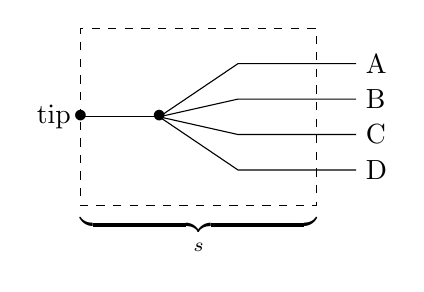
\begin{tikzpicture}[yscale=0.75]
\path (0, 0) coordinate (tip) node{$\bullet$};
\draw (tip) -- ++(1.0,  0.0) coordinate (branch) node{$\bullet$};
\draw (branch) -- ++(1.0,  0.9) -- ++ (1.5, 0) node[right]{A};
\draw (branch) -- ++(1.0,  0.3) -- ++ (1.5, 0) node[right]{B};
\draw (branch) -- ++(1.0, -0.3) -- ++ (1.5, 0) node[right]{C};
\draw (branch) -- ++(1.0, -0.9) -- ++ (1.5, 0) node[right]{D};

%%%%%%%%%%%%%%%%%%%%%%%%%%%%%%%%%%%%%%%%

\node [left] at (tip) {tip};
\draw [dashed]
     (tip)
  -- ++(0, 1.5)
  -- ++(3, 0)
  -- ++(0, -3)
  -- ++(-3, 0) node[pos=0.5, below]{$\underbrace{\hspace{3cm}}_s$}
  -- cycle;

\end{tikzpicture}
\end{center}
%
Since by assumption the candidates in our window are a representative sample
of all chains in the network, this means that \emph{all} chains share this
common prefix, and so we can for \emph{sure} adopt those blocks into our
own chain, moving up our window:
%
\begin{center}
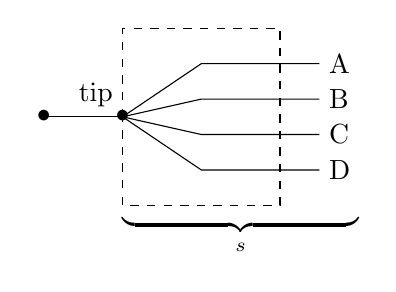
\begin{tikzpicture}[yscale=0.75]
\path (0, 0) coordinate (tip) node{$\bullet$};
\draw (tip) -- ++(1.0,  0.0) coordinate (branch) node{$\bullet$};
\draw (branch) -- ++(1.0,  0.9) -- ++ (1.5, 0) node[right]{A};
\draw (branch) -- ++(1.0,  0.3) -- ++ (1.5, 0) node[right]{B};
\draw (branch) -- ++(1.0, -0.3) -- ++ (1.5, 0) node[right]{C};
\draw (branch) -- ++(1.0, -0.9) -- ++ (1.5, 0) node[right]{D};

%%%%%%%%%%%%%%%%%%%%%%%%%%%%%%%%%%%%%%%%

\node [above left] at (branch) {tip};
\draw [dashed]
     (branch)
  -- ++(0, 1.5)
  -- ++(2, 0)
  -- ++(0, -3)
  -- ++(-2, 0)  node[pos=0.25, below]{$\underbrace{\hspace{3cm}}_s$}
  -- cycle;
\end{tikzpicture}
\end{center}

When we move up the window, we have to wait for it to fill again; we will
discuss this in detail in \cref{genesis:insufficient-blocks}.

\subsection{General case}

Notice that we only adopt blocks when they appear on \emph{all} relevant
chains in the system (\cref{genesis:adopt}). This means that we will never have
to roll such blocks back: everything we adopt we are certain about and will
never change our mind about.

This allows us to generalise the pictures from the previous two sections
slightly. Rather than having the window anchored at genesis, it is
anchored at the tip of a chain of blocks that we are sure about; so for the
fork/discard case (\cref{genesis:discard}), the generalisation looks like
%
\begin{center}
\begin{tikzpicture}[yscale=0.75]
\path (0, 0) coordinate (tip) node{$\bullet$} node[above left]{tip};
\draw (tip) -- ++(1.0,  1.0) coordinate (ab) node{$\bullet$} node[above left]{$ab$};
\draw [dotted] (tip) -- ++(1.5, -0.5) coordinate (cd);
\draw (ab) -- ++(0.5,  0.5) -- ++(2.0, 0) coordinate(A) node[right]{$A$};
\draw (ab) -- ++(0.5, -0.5) -- ++(2.0, 0) node[right]{$B$};
\draw [dotted] (cd) -- ++(0.5,  0.5) -- ++(1.5, 0) node[right]{$C$};
\draw [dotted] (cd) -- ++(0.5, -0.5) -- ++(1.5, 0) node[right]{$D$};
\draw [dashed]
     (tip)
  -- ++(0, 1.75)
  -- ++(3, 0)
  -- ++(0, -3)
  -- ++(-3, 0) node[pos=0.5, below]{$\underbrace{\hspace{3cm}}_{\text{$s$ slots}}$}
  -- cycle;

%%%%%%%%%%%%%%%%%%%%%%%%%%%%%%%%%%%%%%%%

\draw [red, very thick] (tip) -- (ab) -- ++(0.5,  0.5) -- ++(1.5, 0);
\draw (tip) + (-3,0) node{$\bullet$} -- (tip) node[pos=0.5, below]{$\underbrace{\hspace{3cm}}_\text{immutable}$};
\end{tikzpicture}
\end{center}
%
Similarly, for the common prefix/adopt case (\cref{genesis:adopt}), it looks like
%
\begin{center}
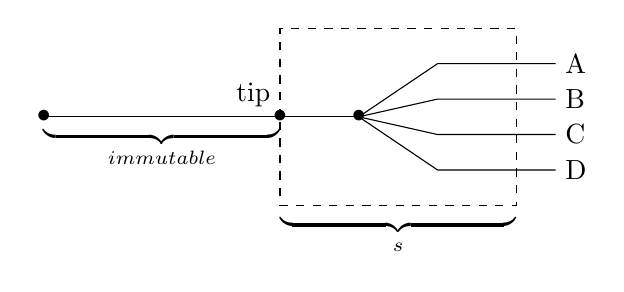
\begin{tikzpicture}[yscale=0.75]
\path (0, 0) coordinate (tip) node{$\bullet$};
\draw (tip) -- ++(1.0,  0.0) coordinate (branch) node{$\bullet$};
\draw (branch) -- ++(1.0,  0.9) -- ++ (1.5, 0) node[right]{A};
\draw (branch) -- ++(1.0,  0.3) -- ++ (1.5, 0) node[right]{B};
\draw (branch) -- ++(1.0, -0.3) -- ++ (1.5, 0) node[right]{C};
\draw (branch) -- ++(1.0, -0.9) -- ++ (1.5, 0) node[right]{D};

%%%%%%%%%%%%%%%%%%%%%%%%%%%%%%%%%%%%%%%%

\node [above left] at (tip) {tip};
\draw [dashed]
     (tip)
  -- ++(0, 1.5)
  -- ++(3, 0)
  -- ++(0, -3)
  -- ++(-3, 0) node[pos=0.5, below]{$\underbrace{\hspace{3cm}}_s$}
  -- cycle;
\draw (tip) + (-3,0) node{$\bullet$} -- (tip) node[pos=0.5, below]{$\underbrace{\hspace{3cm}}_\text{immutable}$};

\end{tikzpicture}
\end{center}

\subsection{Insufficient peers}

When we have not yet connected to at least $\RequiredPeers$ peers, neither of
our two rules can be applied. Consider again the rule that deals with forks:
%
\begin{center}
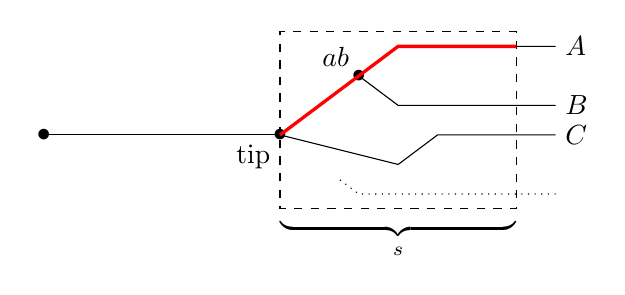
\begin{tikzpicture}[yscale=0.75]
\path (0, 0) coordinate (tip) node{$\bullet$} node[below left]{tip};
\draw (tip) -- ++(1.0,  1.0) coordinate (ab) node{$\bullet$} node[above left]{$ab$};
\draw (tip) -- ++(1.5, -0.5) coordinate (cd);
\draw (ab) -- ++(0.5,  0.5) -- ++(2.0, 0) node[right]{$A$};
\draw (ab) -- ++(0.5, -0.5) -- ++(2.0, 0) node[right]{$B$};
\draw (cd) -- ++(0.5,  0.5) -- ++(1.5, 0) node[right]{$C$};
\path (cd) -- ++(0.5, -0.5) -- ++(1.5, 0) coordinate (D);

\draw [dashed]
     (tip)
  -- ++(0, 1.75)
  -- ++(3, 0)
  -- ++(0, -3)
  -- ++(-3, 0) node[pos=0.5, below]{$\underbrace{\hspace{3cm}}_s$}
  -- cycle;
\draw [dotted] (D) -- ++(-2.5,0) -- ++(-0.25,0.25);

\draw [red, very thick] (tip) -- (ab) -- ++(0.5,  0.5) -- ++(1.5, 0) ;
\draw (tip) + (-3,0) node{$\bullet$} -- (tip);
\end{tikzpicture}
\end{center}
%
Since we don't know the density of the missing chain $D$, it's not sound to
conclude that $A$ is the densest. Similarly, in the rule for a common prefix,
%
\begin{center}
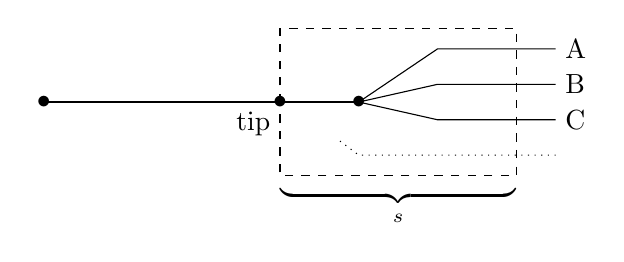
\begin{tikzpicture}[yscale=0.75]
\path (0, 0) coordinate (tip) node{$\bullet$};
\draw (tip) -- ++(1.0,  0.0) coordinate (branch) node{$\bullet$};
\draw (branch) -- ++(1.0,  0.9) -- ++ (1.5, 0) node[right]{A};
\draw (branch) -- ++(1.0,  0.3) -- ++ (1.5, 0) node[right]{B};
\draw (branch) -- ++(1.0, -0.3) -- ++ (1.5, 0) node[right]{C};
\path (branch) -- ++(1.0, -0.9) -- ++ (1.5, 0) coordinate(D);

\draw [dotted] (D) -- ++(-2.5,0) -- ++(-0.25,0.25);
\node [below left] at (tip) {tip};
\draw [dashed]
     (tip)
  -- ++(0, 1.25)
  -- ++(3, 0)
  -- ++(0, -2.5)
  -- ++(-3, 0) node[pos=0.5, below]{$\underbrace{\hspace{3cm}}_s$}
  -- cycle;
\draw (tip) + (-3,0) node{$\bullet$} -- (tip);

\end{tikzpicture}
\end{center}
%
we don't know if the missing chain $D$ \emph{also} starts with the same block,
and so we don't know if the common prefix rule can be applied.

\subsection{Insufficient blocks}
\label{genesis:insufficient-blocks}

We can make more progress in the situation where we \emph{do} have all the peers
we need, but their chains might not fill the look-ahead window. The rule for
common prefix is the simpler case:
%
\begin{center}
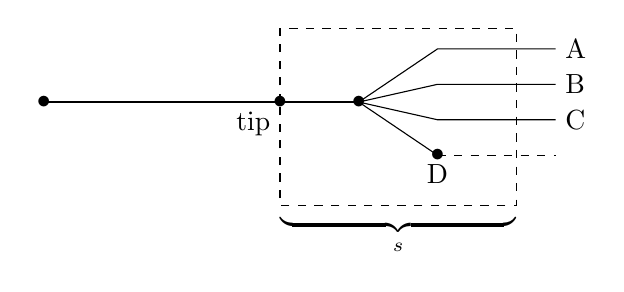
\begin{tikzpicture}[yscale=0.75]
\path (0, 0) coordinate (tip) node{$\bullet$};
\draw (tip) -- ++(1.0,  0.0) coordinate (branch) node{$\bullet$};
\draw (branch) -- ++(1.0,  0.9) -- ++ (1.5, 0) node[right]{A};
\draw (branch) -- ++(1.0,  0.3) -- ++ (1.5, 0) node[right]{B};
\draw (branch) -- ++(1.0, -0.3) -- ++ (1.5, 0) node[right]{C};
\draw (branch) -- ++(1.0, -0.9) coordinate(D) node{$\bullet$} node[below]{D};
\draw [dashed] (D) -- ++ (1.5, 0);

\node [below left] at (tip) {tip};
\draw [dashed]
     (tip)
  -- ++(0, 1.25)
  -- ++(3, 0)
  -- ++(0, -3)
  -- ++(-3, 0) node[pos=0.5, below]{$\underbrace{\hspace{3cm}}_s$}
  -- cycle;
\draw (tip) + (-3,0) node{$\bullet$} -- (tip);

\end{tikzpicture}
\end{center}
%
Even though we have not yet seen enough of chain $D$ to fill the window, it does
not matter; by assumption, if we see at least $\RequiredPeers$ chains, we have
seen all relevant chains in the network, and if all of those chains start with
the same block, we can definitely adopt that block. From a practical
perspective, this is an important special case: under normal circumstances, we
expect all peers in the network to report the exact same chain, at least for all
but the last few of the millions of blocks on their chains. This means that we
can adopt blocks almost as soon as we see them during syncing.

\pagebreak

The situation is more subtle in the case of a fork:
%
\begin{center}
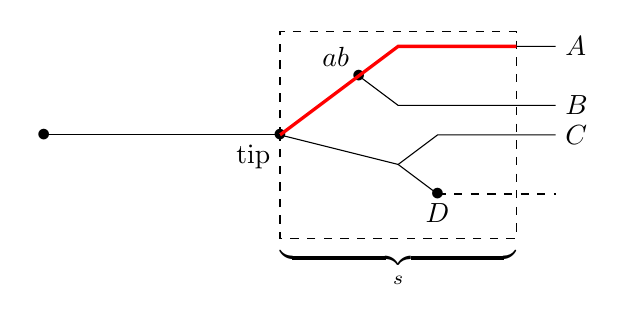
\begin{tikzpicture}[yscale=0.75]
\path (0, 0) coordinate (tip) node{$\bullet$} node[below left]{tip};
\draw (tip) -- ++(1.0,  1.0) coordinate (ab) node{$\bullet$} node[above left]{$ab$};
\draw (tip) -- ++(1.5, -0.5) coordinate (cd);
\draw (ab) -- ++(0.5,  0.5) -- ++(2.0, 0) node[right]{$A$};
\draw (ab) -- ++(0.5, -0.5) -- ++(2.0, 0) node[right]{$B$};
\draw (cd) -- ++(0.5,  0.5) -- ++(1.5, 0) node[right]{$C$};
\draw (cd) -- ++(0.5, -0.5) coordinate(D) node{$\bullet$} node[below]{$D$};
\draw [dashed] (D) -- ++ (1.5, 0);

\draw [dashed]
     (tip)
  -- ++(0, 1.75)
  -- ++(3, 0)
  -- ++(0, -3.5)
  -- ++(-3, 0) node[pos=0.5, below]{$\underbrace{\hspace{3cm}}_s$}
  -- cycle;

\draw [red, very thick] (tip) -- (ab) -- ++(0.5,  0.5) -- ++(1.5, 0) ;
\draw (tip) + (-3,0) node{$\bullet$} -- (tip);
\end{tikzpicture}
\end{center}
%
We might only be seeing a prefix of $D$'s chain, or it might be that $D$'s chain
simply isn't longer. Fortunately, $D$ will report its tip as part of the chain
sync protocol.\footnote{In principle, making use of this information is not
critical: we could assume the node always has more headers and simply wait,
timing out if they don't give us more headers. We don't currently have such a
timeout---we time out only if a node tells us they have more header but then
fail to provide them to us---and even if we did, it would mean introducing
unnecessary delays into chain selection: if we happen to connect to an upstream
peer that is not up to date, we would be dependent on a timeout before we can
rule this peer out.} We can use this information to distinguish between these
cases:
%
\begin{itemize}
\item If $D$ reports that its tip is \textbf{within} our $s$ window, then the
chain simply isn't any longer. This case is subtle. If the intersection between
$D$ and the tip is less than $s$, the genesis rule tells us to look at chain
length, but of course chain length changes over time (unlike an intersection
point between two chains and the density at that intersection point), and so we
cannot make conservative decisions based on it.

We said in the introduction that we can switch from conservative mode to
speculative mode $s$ slots from the wall clock \emph{at the latest}: otherwise
the chains \emph{cannot} fill the window. Now we see that actually we need to
switch \emph{sooner}, at $s + x$ slots from the wall clock.

\begin{center}
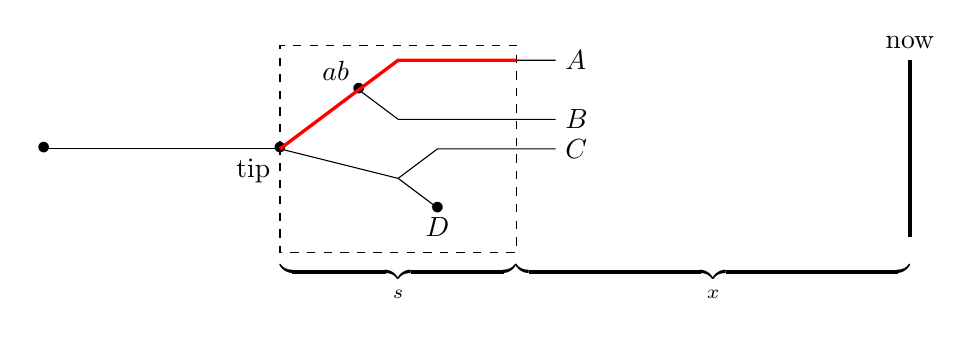
\begin{tikzpicture}[yscale=0.75]
\path (0, 0) coordinate (tip) node{$\bullet$} node[below left]{tip};
\draw (tip) -- ++(1.0,  1.0) coordinate (ab) node{$\bullet$} node[above left]{$ab$};
\draw (tip) -- ++(1.5, -0.5) coordinate (cd);
\draw (ab) -- ++(0.5,  0.5) -- ++(2.0, 0) node[right]{$A$};
\draw (ab) -- ++(0.5, -0.5) -- ++(2.0, 0) node[right]{$B$};
\draw (cd) -- ++(0.5,  0.5) -- ++(1.5, 0) node[right]{$C$};
\draw (cd) -- ++(0.5, -0.5) coordinate(D) node{$\bullet$} node[below]{$D$};

\draw [dashed]
     (tip)
  -- ++(0, 1.75)
  -- ++(3, 0)
  -- ++(0, -3.5)
  -- ++(-3, 0) node[pos=0.5, below]{$\underbrace{\hspace{3cm}}_s$}
  -- cycle;

\draw [red, very thick] (tip) -- (ab) -- ++(0.5,  0.5) -- ++(1.5, 0) ;
\draw (tip) + (-3,0) node{$\bullet$} -- (tip);

%
\draw [ultra thick] (8,-1.5) -- (8,1.5) node[above]{now};
\node at (5.5, -2.25) {$\underbrace{\hspace{5cm}}_x$};
\end{tikzpicture}
\end{center}

We should pick $x$ such that if a node reports that its tip is within our
look-ahead window, and is therefore $x + n$ away from the wall clock,
for some $0 \le n < s$, we can conclude that the node is \emph{itself} not
up to date with the chain (it is itself still syncing) and we can disconnect
from it (perhaps we will reconnect to it again later).

On the other hand, we must pick $x$ such that the probability of seeing more
than $k$ blocks in $s + x$ is still negligibly small, so that we are not
switching too soon. A good choice might be $x$ somewhere between $s$ and $2s$,
i.e., switching from conservative mode to speculative mode once we are between
$2s$ and $3s$ slots away from the wallclock (that is, roughly $\frac{1}{4}k$ and
$\frac{1}{2}k$ blocks); see also \cref{genesis:switch-over-point}.

\item If the node reports that its tip is \textbf{outside} the $s$ window, we
must wait until we have seen enough of $D$'s chain to fill the window before we
can say something conclusive about $D$'s density. Note that if $D$ reports a tip
outside the window but then doesn't send us any more headers, we will eventually
time-out and disconnect from $D$, protecting us from a DoS attack.
\item There is one exception to the previous case: if we have not yet seen all
of $D$'s chain, but the part that we \emph{did} see (and validated) already
contains more blocks than another chain (say $A$), we can safely conclude
that $D$ must be denser than $A$ (provided we \emph{have} seen enough of $A$
to fill the window).
\end{itemize}

Since not every slot on the chain contains a block, it is not entirely trivial
to detect whether we have seen enough of a chain to fill the window; we must
wait until we have seen the first block in or after the last slot of the window:
%
\begin{center}
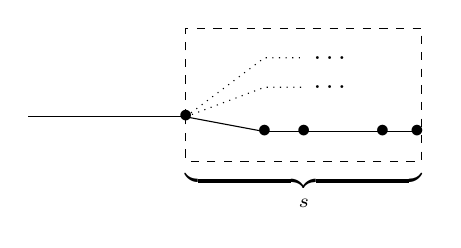
\begin{tikzpicture}[yscale=0.75,baseline=0pt]
\draw (0,0) -- (2,0) node{$\bullet$} coordinate (tip);
\draw [dotted] (tip) -- ++(1,1) -- ++ (0.5,0) node[right]{$\ldots$};
\draw [dotted] (tip) -- ++(1,0.5) -- ++ (0.5,0) node[right]{$\ldots$};
\draw (tip) -- ++(1,-0.25) node {$\bullet$} coordinate (a);
\draw (a) -- ++(0.5,  0) node {$\bullet$} coordinate (b);
\draw (b) -- ++(1.0,  0) node {$\bullet$} coordinate (c);
\draw (c) -- ++(0.5, 0) node [left=-0.15cm] {$\bullet$};
\draw [dashed]
     (tip)
  -- ++(0, 1.5)
  -- ++(3, 0)
  -- ++(0, -2.25)
  -- ++(-3, 0) node[pos=0.5, below]{$\underbrace{\hspace{3cm}}_s$}
  -- cycle;
\end{tikzpicture}
%
\qquad or \qquad
%
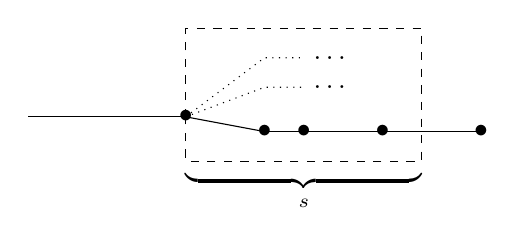
\begin{tikzpicture}[yscale=0.75,baseline=0pt]
\draw (0,0) -- (2,0) node{$\bullet$} coordinate (tip);
\draw [dotted] (tip) -- ++(1,1) -- ++ (0.5,0) node[right]{$\ldots$};
\draw [dotted] (tip) -- ++(1,0.5) -- ++ (0.5,0) node[right]{$\ldots$};
\draw (tip) -- ++(1,-0.25) node {$\bullet$} coordinate (a);
\draw (a) -- ++(0.5,  0) node {$\bullet$} coordinate (b);
\draw (b) -- ++(1.0,  0) node {$\bullet$} coordinate (c);
\draw (c) -- ++(1.25, 0) node {$\bullet$};
\draw [dashed]
     (tip)
  -- ++(0, 1.5)
  -- ++(3, 0)
  -- ++(0, -2.25)
  -- ++(-3, 0) node[pos=0.5, below]{$\underbrace{\hspace{3cm}}_s$}
  -- cycle;
\end{tikzpicture}
\end{center}

\section{Partial validation}

Everything we have discussed so far was in terms of headers. In particular,
we \emph{discard} chains based on header validity only. This is justified,
because the argument that the honest chain must be denser depends on checking
the \emph{leadership schedule} only: as long as we verify headers, thereby
verifying that those headers were produced by nodes that were indeed selected
leader in those slots, we have verified that leadership schedule; whether or
not the rest of the block is valid is not relevant.

Of course, if we skip header validation altogether, then it would be all too
trivial for an attacker to present us with a very dense chain, causing us to
disconnect from the honest chain. This means that if  the genesis chain
selection rule is implemented along the lines sketched in this chapter, header
validation during chain sync is critical.

We only \emph{adopt} blocks (or rather, present them to the chain database) when
\emph{all} chains share those blocks. Before we adopt these blocks into our own
chain (indeed, before we adopt \emph{any} block) we validate them; if such a
block, shared by all chains we are aware off, turns out to be invalid, something
went horribly wrong. Perhaps we got eclipsed by an attacker after all, and they
are presenting us with an invalid block as some form of DoS attack. It is
unclear what to do in this situation; we might not have much choice other than
to wipe the entire chain database and start afresh with an empty chain and a
fresh set of peers.

\section{Switching between modes}
\label{genesis:switching-modes}

Let's consider the easiest case first. When a new node joins the network, its
local chain still empty, they check their clock, notice that they are more than
$k$ blocks away from the currently longest chain
(\cref{genesis:switch-over-point}), and so use conservative chain selection
mode, adding blocks to their chain only once they are sure about them. Once they
get near the tip of the chain, they switch to speculative mode.

In a sense this is how the genesis paper envisions the genesis rule to be used:
new nodes can join the network at any stage, \emph{and then stay up to date}.
In reality, however, it is entirely possible for a node that is currently up
to date to fall behind; the reason might be as simple as a user putting
their computer to sleep for a few days. We must therefore be able to go
\emph{back} from speculative mode into conservative mode.

In the discussion of the rules above, we assumed that our look-ahead window
was anchored at the tip of a chain of blocks we were sure about. To bring us
back to this situation when we switch out of speculative mode, we should
anchor the look-ahead window at the tip of our immutable database (i.e.,
$k$ blocks back from our current tip), and then proceed as above.

When we anchor the look-ahead window at our immutable tip, \emph{this does not
have to affect our current chain}. We anchor the window at the immutable tip,
then start going forward, offering blocks to the chain database as we make
progress. In most cases, most (if not all) blocks that we decide we can be sure
about will be shared by our current chain, so nothing changes. If \emph{all}
blocks are shared, at some point our chain will simply start to grow again. If
only a prefix is shared, at some point the new chain that we are constructing
will be preferred over our own (using normal chain selection) and we will switch
to it at that point. At most this would involve a roll-back of $k$, because
that's where we anchored our look-ahead window initially, so that is the
earliest point at which an alternative chain could fork off.

\section{Miscellaneous other remarks}

\subsection{The original genesis rule}
\label{genesis:original}

The genesis rule as defined in \cref{genesis:rule} is a minor variation on
the rule as presented in the paper \cite{cryptoeprint:2018:378}, although
the two rules are equivalent in terms of the security of the system
[Badertscher, personal communication]. The original rule is shown in
\cref{genesis:maxvalid-bg}, and paraphrased below:

\begin{definition}[Genesis chain selection rule, original version]
\label{genesis:originalrule}
A candidate chain is preferred over our current chain if

\begin{itemize}
\item The intersection between the candidate chain and our chain is \textbf{no
more than $k$} blocks back, and the candidate chain is strictly \textbf{longer}
than our chain.

\item If the intersection \emph{is} \textbf{more than $k$} blocks back, and the
candidate chain is \textbf{denser} (contains more blocks) than our chain in
a region of $s$ slots starting at the intersection.
\end{itemize}
\end{definition}

This version of the rule is less suitable for our purposes, for two reasons.
First, consider once more the rule for forks during conservative chain
selection:
%
\begin{center}
\begin{tikzpicture}[yscale=0.75]
\path (0, 0) coordinate (tip) node{$\bullet$} node[below left]{tip};
\draw (tip) -- ++(1.0,  1.0) coordinate (ab) node{$\bullet$} node[above left]{$ab$};
\draw [dotted] (tip) -- ++(1.5, -0.5) coordinate (cd);
\draw (ab) -- ++(0.5,  0.5) -- ++(2.0, 0) coordinate(A) node[right]{$A$};
\draw (ab) -- ++(0.5, -0.5) -- ++(2.0, 0) node[right]{$B$};
\draw [dotted] (cd) -- ++(0.5,  0.5) -- ++(1.5, 0) node[right]{$C$};
\draw [dotted] (cd) -- ++(0.5, -0.5) -- ++(1.5, 0) node[right]{$D$};
\draw [dashed]
     (tip)
  -- ++(0, 1.75)
  -- ++(3, 0)
  -- ++(0, -3)
  -- ++(-3, 0) node[pos=0.5, below]{$\underbrace{\hspace{3cm}}_{\text{$s$ slots}}$}
  -- cycle;

%%%%%%%%%%%%%%%%%%%%%%%%%%%%%%%%%%%%%%%%

\draw [red, very thick] (tip) -- (ab) -- ++(0.5,  0.5) -- ++(1.5, 0);
\end{tikzpicture}
\end{center}
%
We know that the distance from $A \ldots D$ to the anchor of the window is at
least $s$ slots. However, in order to be able to apply the \emph{original}
genesis rule as stated, that is not sufficient. We would need to know if the
distance to that intersection point is at least $k$ blocks in order to know
if we should be comparing density or chain length. This means we would need to
make our look-ahead window significantly larger, so that we don't just wait
until we have seen at least $s$ slots, but also wait until we know for sure
if the tips of various chains we are considering at at least $k$ blocks away
from the intersection point.

The second reason that this rule is less suitable for us is that it has an odd
corner case. Consider the following situation, where we have two chains $A$
and $B$; $A$ is denser than $B$ at the intersection with $B$, but $B$
is longer:
%
\begin{center}
\begin{tikzpicture}
\path (0, 0) coordinate (tip) node{$\bullet$};
\draw (tip) -- ++(1.0,  0.5) -- ++(2.5, 0) coordinate(C1) node[right]{$A$};
\draw (tip) -- ++(1.0, -0.5) -- ++(3.5, 0) coordinate(C2) node[right]{$B$};
\draw [red, very thick] (tip) -- ++(1.0,  0.5) -- ++(2.0, 0);
\draw [dashed]
     (tip)
  -- ++(0, 0.75)
  -- ++(3, 0)
  -- ++(0, -1.5)
  -- ++(-3, 0) node[pos=0.5, below]{$\underbrace{\hspace{3cm}}_{\text{$s$ slots}}$}
  -- cycle;
\path (tip) -- (C1) node[pos=0.5, above=0.5cm]{$\overbrace{\hspace{3.5cm}}^{\text{fewer than $k$ blocks}}$};
\path (tip) -- (C2) node[pos=0.5, below=1.1cm]{$\underbrace{\hspace{4.5cm}}_{\text{more than $k$ blocks}}$};
\draw (tip) + (-3,0) node{$\bullet$} -- (tip);
\end{tikzpicture}
\end{center}
%
If our current chain is $A$, then the intersection point with $B$ is \emph{less}
than $k$ blocks back, so the rule says we should prefer $B$, because it is the
longer chain. But if our current chain is $B$, then the intersection point with
$A$ is \emph{more} than $k$ blocks back, and so the rule says we should prefer
$A$, because it is denser!

The rule as formulated in the paper (reproduced here
in \cref{genesis:maxvalid-bg}) does not suffer from this ``flip-flop''
behaviour, but only because it considers chains strictly in order. If the list
of chains $\mathcal{N} = \{ A, B \}$, we end up choosing $B$, and if that list
is $\mathcal{N} = \{ B, A \}$, we end up choosing $A$.

Perhaps this is not a problem in speculative mode; we just pick \emph{an} order,
choosing either $A$ or $B$, and eventually settle on $A$ once it becomes long
enough. However, it is problematic in conservative mode where we want
definitive answers.

\begin{figure}
\hrule

\textbf{Parameters} \\[0.5em]
\begin{tabular}{ll}
$C_\mathit{loc}$ & Current chain \\
$\mathcal{N} = \{C_1, \ldots, C_M\}$ & All possible chains (including our own) \\
$k$ & Security parameter (\cref{consensus:overview:k}) \\
$s$ & Genesis window size (Genesis rule specific parameter) \\
$f$ & Active slot coefficient (\cref{praos:f}) \\[1em]
\end{tabular}

\textbf{Algorithm}

\begin{lstlisting}[escapeinside={(*}{*)}, language={}, keywords={for,do,if,then,else,end,return}]
// Compare (*$C_\mathit{max}$*) to each (*$C_i \in \mathcal{N}$*)
Set (*$C_\mathit{max} \leftarrow C_\mathit{loc}$*)
for (*$i = 1$*) to (*$M$*) do
  if (*$(C_i \text{ forks from } C_\mathit{max} \text{ at most } k \text{ blocks})$*) then
    if (*$|C_i| > |C_\mathit{max}|$*) then // Condition A
      Set (*$C_\mathit{max} \leftarrow C_i$*).
    end if
  else
    Let (*$j \leftarrow \max \Bigl\{ j' \ge 0 \mathrel{\Bigl\lvert} C_\mathit{max} \text{ and } C_i \text{ have the same block in } \mathtt{sl}_{j'} \Bigr\} $*)
    if (*$|C_i[0 : j + s]| > |C_\mathit{max}[0 : j + s]|$*) then // Condition B
      Set (*$C_\mathit{max} \leftarrow C_i$*).
    end if
  end if
end for
return (*$C_\mathit{max}$*)
\end{lstlisting}

\hrule
\caption{\label{genesis:maxvalid-bg}Algorithm \texttt{maxvalid-bg}}
\end{figure}

\subsection{Switching to shorter chain}

When we introduced chain selection in \cref{consensus:overview:chainsel}, we
stated an invariant that we never switch to a shorter chain
(\cref{never-shrink}). The most important rationale for this invariant is that
if we \emph{did} switch to a shorter chain, and then continue to support a
maximum rollback of $k$ blocks, we would effectively end up having to
support infinite rollback.

When we support genesis, we must relax this invariant slightly. The genesis
rule means that we \emph{might} switch to a shorter chain, if it is denser
than our current chain at the intersection point. This isn't a problem per se,
provided that when it happens our maximum rollback temporarily shrinks, until
we have seen a sufficient amount of blocks on the new chain.

As discussed in \cref{genesis:original}, the genesis rule as stated in the
paper is slightly different from the one we use here. Moreover, the paper
also shows \cite[Theorem 2]{cryptoeprint:2018:378} that we only need to
look at density when we are not up to date, and can simply look at length
otherwise. It is therefore tempting to think that we could use that theorem
to avoid switching to a shorter chain. However, recall that we also need to do
chain selection when we switch back from speculative mode to conservative mode,
which happens precisely when we are \emph{not} up to date
(\cref{genesis:switching-modes}).\footnote{Alternatively, we could roll back to
the tip of our immutable database when we switch to conservative mode, but if we
did, we would \emph{definitely}  be switching to a shorter chain, of course.}

These problems may well have solutions: perhaps if we
%
\begin{enumerate}
\item use the longest chain rule in speculative mode (or,
equivalently, the genesis rule as it was phrased in the paper, along with
Theorem 2 of the paper),
\item use our (alternative) genesis rule in conservative mode
\item have an argument (proof sketch) that when we do switch from speculative
back to conservative mode, it is sound to switch to the (potentially) new chain
only once it's longer than our own
\end{enumerate}
%
we could avoid ever switching to a shorter chain. This would seem considerably
more ad hoc than what we have proposed in this chapter, however.

\subsection{Equal density}

If in conservative mode we have two forks branching at the start of the window,
and they have exactly the same density, we need a tie-breaker in order to be
able to make progress. The genesis paper does not prefer either chain in such
a scenario, switching only if another chain is strictly denser. We can therefore
follow suit, and just discard one of the two chains randomly.

\subsection{Switch-over point}
\label{genesis:switch-over-point}

Theorem 2 of the genesis paper says that when we are up to date, we do not have
to roll back more than $k$ blocks. At least, that is how Christian Badertscher
rephrased the theorem in his presentation\footnote{``Ouroboros Genesis:
Composable Proof-of-Stake Blockchains with Dynamic Availability'', published by
the ACM, \url{https://www.youtube.com/watch?v=m-kI_Sb8oII}}. He does not specify
in the presentation what ``up to date'' means, exactly, and unfortunately the
theorem as stated in the paper (never mind its proof) is impenetrable to mere
mortals. In this chapter we have interpreted it to mean ``the tip of our ledger
is within $k$ blocks of the longest chain in the network''.\todo{Verify}

As mentioned in the introduction, the latest point we \emph{can} switch is when
we are $s$ slots away from the wallclock. Any later, and we would not be able to
fill our look-ahead window. In \cref{genesis:insufficient-blocks} we
saw that in practice we will want to switch sooner; there we suggested that
we might switch once we are within $2s$ slots from the wallclock.

Provided that the above interpretation of ``up to
date'' is correct, then switching from conservative mode to speculative mode
when we are $s + x$ slots away from the wallclock would be unsound only if those $s + x$
slots contain \emph{more} than $k$ blocks (fewer would mean that we could have
switched earlier). If we use the default genesis window of $s = \frac{1}{4}(k /
f)$ (\cref {default-genesis-window}), and set $x = s$, then for Cardano
($f = 0.05$ and $k = 2160$) we get
%
\begin{equation*}
\sum_{i = k + 1}^{2s}  {{2s} \choose i} \times f^i \times (1 - f)^{{2s} - i}
\approx 1.4379 \times 10^{-196}
\end{equation*}
%
and if we pick $x = 2s$ (i.e., switch when we are $3s$ slots away from the
wallclock), we get $9.4367 \times 10^{-40}$. Both of these probabilities are
negligibly small.

Deciding exactly where to draw a line in the sand and decide what the largest
probability is that we still consider negligible is of course difficult. We
might look for some comparison points; for example, the probability of correctly
guessing a random 256-bit key is $2 ^ {-256} = (10 ^ {\log_{10} 2})^{-256} = 10
^ {\log_{10} 2 \times -256} \approx 10^{-77}$; we could also compare to the
probability of random bit flips (for example, see \cite{6468485}).
Alternatively, we could compute how long it would take for a problem to arise;
the Algorand paper does such a calculation \cite{chen2017algorand} and comes to
a conclusion that a probability of $10^{-18}$ would still be fine for a decision
that is made every second; if we take that as a lower bound, the earliest we
could switch to speculative mode is roughly $3.3s$ slots from the wallclock.

\subsection{Possible optimisations}

Doing chain selection in conservative mode might open the door to a number
of performance optimisations. Here we just list some of the possibilities:

\begin{itemize}

\item When a node is operational, we try to line up its average-case performance
requirements with its worst-case performance requirements, since this avoids
an attack vector: if the average-case performance would be significantly better
than the worst-case, it is likely that nodes would be optimised for the average
case (for instance, run on hardware that can handle the average case, but not
necessarily the worst case); then if a malicious node can intentionally cause
the worst-case, they might be able to bring down parts of the network.

For this reason we don't normally share work between various peers; when
multiple upstream peers all send us the same header, we verify the header
each time. This means that the average case (most upstream chains are the same)
and the worst case (every upstream chain is different) are equal.

However, it is less important that we can predict accurately how long it takes
a node (that isn't up to date) to sync with the network. Such a node is anyway
not producing blocks; here, faster is simply better. This means that while we
are in conservative chain selection mode, we could share the validation work
across upstream peers: when two peers send us the same header, we do not need
to validate it twice.

This is \emph{especially} important during conservative mode, because due to the
requirement to have at least $\RequiredPeers$ upstream peers, we might be
connecting to more peers than usual. Moreover, under normal circumstances we
expect all of these peers to present us with exactly the same chain (and
finally, these cryptographic checks are expensive).

\item Similarly, since we expect all upstream nodes to report the same chain,
if we receive a bunch of headers from peer 1, we can just ask peer 2
whether they have the most recent of those headers on their chain, thereby
skipping over large chunks of the chain altogether.

\item Since we only ever fetch blocks strictly in order, we can simplify
the interaction with the block fetch client: it might be easier to generate
longer fetch ranges, as well as spread the load more evenly across the peers.

\item Since we only adopt blocks we are sure about during conservative mode,
it might be possible to bypass the volatile database entirely. However,
how this works when we switch back from speculative mode to conservative mode
would require careful thought.

\item Since we switch to conservative mode when we are more than $s$ slots away
from the wall clock, and only adopt blocks in conservative mode that we never
roll back, it is possible that the maximum roll back we have to support
is in fact less than $k$. This too would require careful consideration.

\end{itemize}

\subsection{TODOs}

TODOs\todo{TODO}:

\begin{itemize}
\item Should we look at the immutable tip or the volatile tip to determine if we
are in genesis mode? The immutable tip seems appealing (after all, that's what
we mean when we say everybody has been up to date and shares a common prefix),
but it feels dangerous to me: we might be hovering near the edge of that window,
dropping in and out of conservative mode even during normal operation.
\item Add definition of ``conservative'' decision somewhere:
decisions that we will never have to revisit. in other words, a conservative
decision to adopt a block is a block that we know we want on our chain, we will
never switch to a fork that doesn't contain that block; and likewise, a
conservative decision to discard chain is one in which we cannot later discover
that actually we did want (a prefix of) that chain after all.
\item Think about how to deal with rollback (from other nodes) whilst we are
in conservative mode.
\end{itemize}
